%!TEX root = ../Thesis.tex
\chapter{系统架构总体设计}\label{chap:architecture}

本章将详细阐述基于 FPGA 的 SLAM 后端加速器的系统级架构设计。本系统选用赛灵思（Xilinx）Zynq 系列 SoC 作为核心计算平台，该平台通过高性能 AXI 总线将处理器系统（PS）与可编程逻辑（PL）紧密耦合，为软硬协同设计提供了物理基础。在开发流程上，采用 Vivado 工具套件进行硬件逻辑架构设计与综合，利用 Vitis 统一软件平台进行嵌入式驱动与应用开发，并通过 DMA 引擎实现 PS 与 PL 之间的高带宽数据交互。

在此硬件基础之上，本章将依次论述系统的总体设计目标、软硬件功能的详细划分策略，以及连接软硬件两侧的数据流与通信协议设计。

\section{总体设计目标}

针对嵌入式自主移动平台对 SLAM 系统在实时性、能耗以及精度方面的严苛要求，本文设计的基于 FPGA 的后端加速器旨在通过软硬协同的设计思路，突破传统通用处理器的计算瓶颈。系统的总体设计目标主要包含以下四个方面：

\begin{enumerate}
    \item \textbf{高实时性需求}：实时性是 SLAM 系统实现在线定位的关键指标。为了配合视觉前端的高频采样并确保控制回路的稳定性，本系统设计的后端加速器需实现在滑动窗口负载下，单次非线性优化的频率稳定在 \textbf{25~Hz 以上}。这意味着系统必须在 40~ms 内完成包括雅可比（Jacobi）矩阵生成、海森（Hessian）矩阵累加及舒尔补（Schur Complement）消元在内的所有复杂矩阵运算。

    \item \textbf{低功耗与高能效比}：嵌入式平台（如无人机、手持 AR 设备）对续航时间极其敏感。本设计的目标是在维持高性能计算输出的同时，满足移动端的低功耗限制。通过利用 FPGA 的硬件定制特性，引入动态门控机制跳过无效计算，旨在实现显著优于通用嵌入式处理器（如 ARM Cortex-A 系列）的\textbf{能效比（Performance per Watt）}。

    \item \textbf{高定位精度维持}：硬件加速器的引入不应以牺牲定位精度为代价。由于 FPGA 硬件实现中通常涉及定点化（Fixed-point）处理，本系统的设计目标是优化位宽分配与运算溢出控制，确保经硬件加速后的后端优化结果（位姿轨迹与路标点坐标）与原始双精度浮点全软件实现相比，其误差保持在极小范围内，维持系统原有的\textbf{定位精度等级}。

    \item \textbf{资源利用率最优化}：本文采用的 Zynq UltraScale+ 系列 FPGA 片上资源（如逻辑单元 LUT、乘法器 DSP、块存储 BRAM）相对有限。因此，设计目标之一是实现计算逻辑的紧凑化。通过复用计算单元、优化 Hessian 矩阵的存储结构（如隐式索引机制）以及精简数据流水线，确保核心加速算子能够被适配到\textbf{资源受限的嵌入式 SoC} 中。
\end{enumerate}

\section{软硬件功能划分}

为了在 Zynq 异构 SoC 平台上实现最优的性能与能效平衡，本文遵循将计算密集型任务迁移至硬件、逻辑管理型任务保留在软件的设计原则，对系统进行了深度的软硬件功能划分。系统整体分为处理器系统（Processing System, PS）端与可编程逻辑（Programmable Logic, PL）端两大部分，如图~\ref{fig:hw_sw_partition}~所示。

\begin{figure}[htbp]
    \centering
    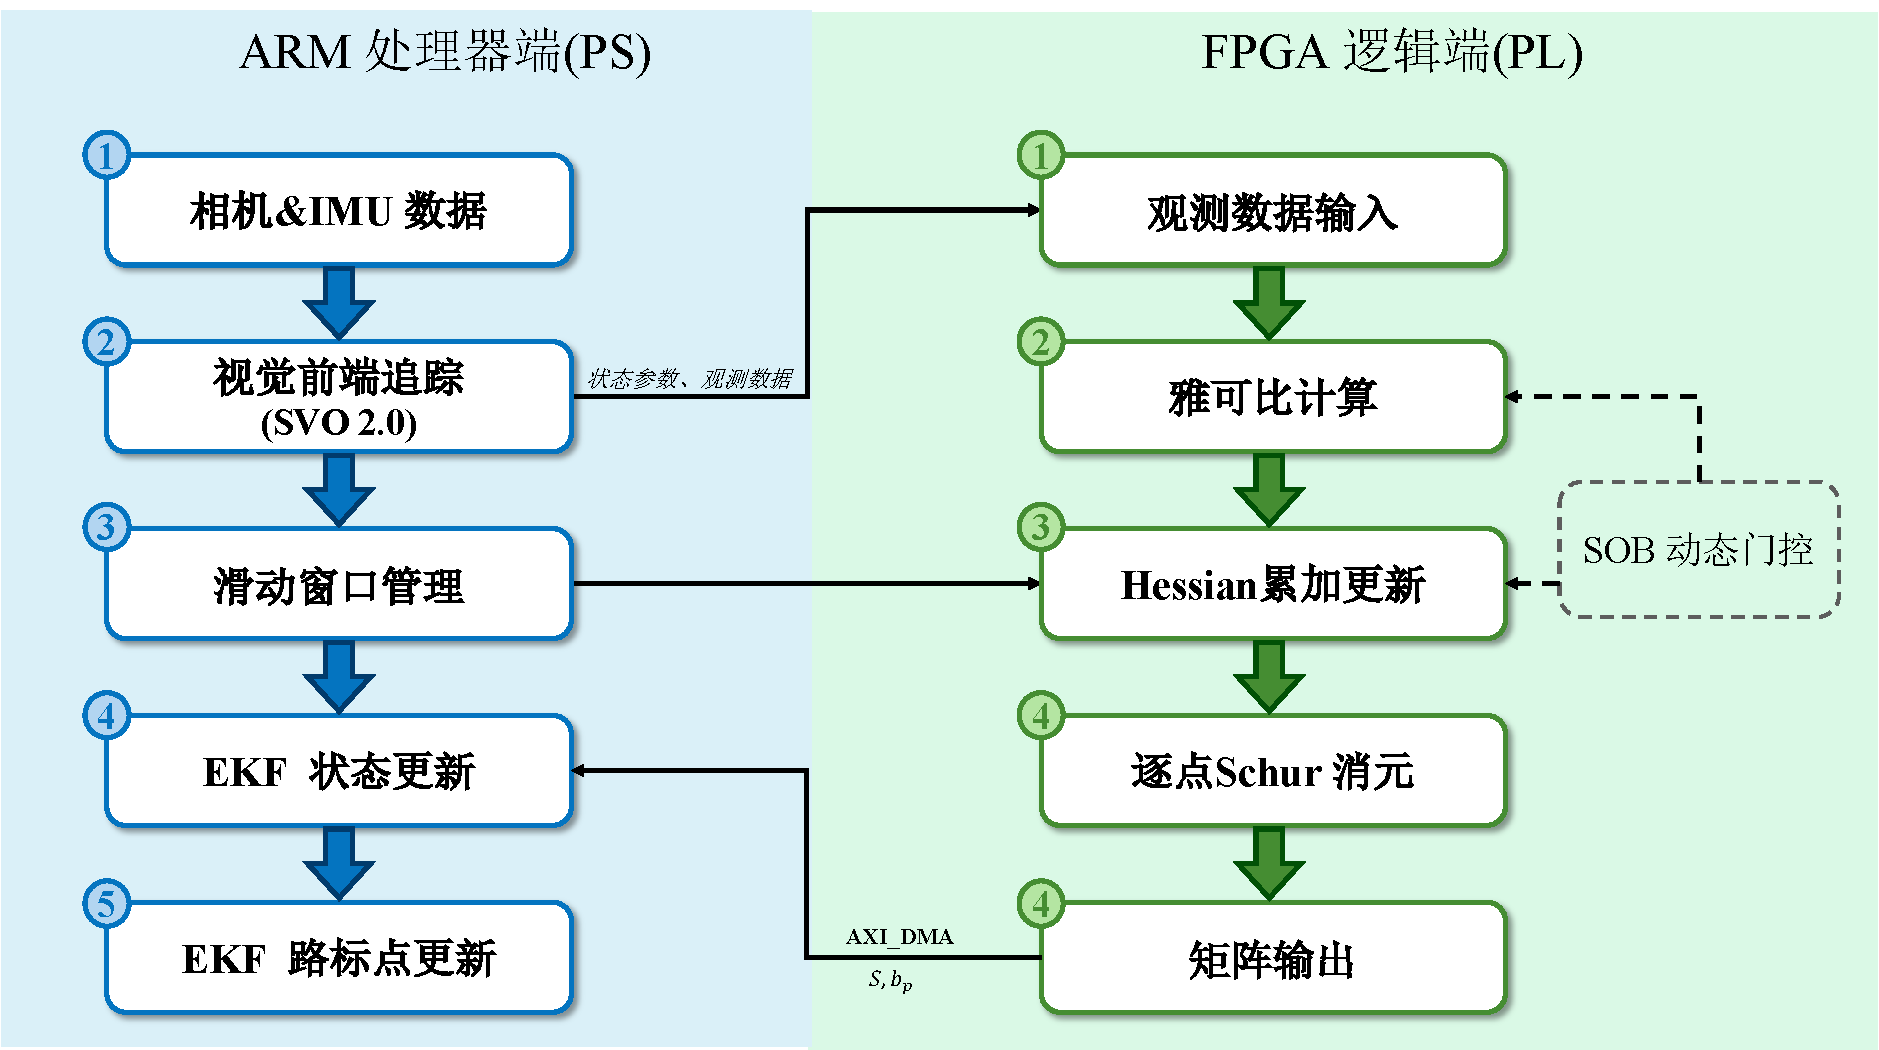
\includegraphics[width=0.95\textwidth]{Img/hw_sw_partition.pdf}
    \bicaption{软硬件功能划分与数据流示意图}{Hardware-Software Functional Partitioning and Data Flow Diagram}
    \label{fig:hw_sw_partition}
\end{figure}

\subsection{ARM 处理器端（PS）任务}

ARM 处理器端主要负责系统的全局协调、低频逻辑评估以及对外部传感器的管理，重点执行具有高逻辑分歧度的非加速任务。其具体任务包括：

\subsubsection{数据获取与多源同步}

系统通过驱动程序实时采集来自双目相机的图像流与惯性测量单元（IMU）的原始加速度计和陀螺仪数据。由于视觉传感器与惯性传感器的采样频率和触发机制存在异步特性（相机通常工作在 20--30~Hz，IMU 则高达 200--400~Hz），系统需要在 PS 端实现精确的时间戳对齐与数据缓冲管理。具体实现上，采用基于硬件时钟的时间戳标注机制，并使用线性插值方法同步异步数据流，确保后续前端追踪与后端优化的观测数据具有时序一致性。

\subsubsection{视觉前端追踪}

本系统采用 SVO 2.0~\cite{forster2017svo} 作为视觉前端，实现快速鲁棒的特征提取与帧间追踪。SVO 2.0 是一种半直接单目视觉里程计（Semi-Direct Monocular Visual Odometry），结合了直接法的快速性与特征法的鲁棒性。其核心工作流程包括以下几个关键步骤：

\paragraph{特征提取与初始化}
系统在新到达的关键帧上执行 FAST（Features from Accelerated Segment Test）角点检测算法，提取图像中具有显著灰度变化的角点特征。为保证特征点在图像上的均匀分布，采用自适应非极大值抑制（Adaptive Non-Maximal Suppression, ANMS）策略，将图像划分为均匀网格并限制每个网格内的特征点数量上限。提取出的特征点被初始化为候选路标点，并建立对应的深度滤波器。

\paragraph{深度滤波与三角化}
由于单目相机缺乏直接的深度信息，系统采用贝叶斯深度滤波器对每个新特征点的逆深度进行概率估计。具体而言，对每个特征点维护一个高斯分布 $\mathcal{N}(\rho, \sigma^2)$，其中 $\rho$ 为逆深度均值，$\sigma^2$ 为不确定性。随着该特征点在后续帧中被持续观测，利用三角测量的几何约束对深度分布进行贝叶斯更新，直至不确定性 $\sigma^2$ 收敛到预设阈值以下，此时该特征点被正式提升为成熟路标点并参与后端优化。

\paragraph{直接法特征对齐}
SVO 2.0 采用基于光度一致性的直接法进行帧间运动估计。对于已跟踪的特征点，系统在当前帧中以其预测投影位置为中心，通过最小化光度残差（Photometric Residual）优化特征点在新帧中的精确像素坐标：
\begin{equation}
    \min_{\mathbf{u}} \sum_{i \in \mathcal{P}} \| I_{\text{ref}}(\mathbf{u}_i) - I_{\text{cur}}(\mathbf{u}_i + \Delta \mathbf{u}) \|^2
\end{equation}
其中 $I_{\text{ref}}$ 和 $I_{\text{cur}}$ 分别为参考帧和当前帧的灰度图像，$\mathcal{P}$ 为特征点邻域的像素集合，$\Delta \mathbf{u}$ 为像素级的位移增量。直接法避免了传统特征描述子的计算开销，显著提升了前端处理速度。

\paragraph{关键帧选择策略}
为防止关键帧冗余并确保滑动窗口内的帧间约束充分，系统采用基于场景覆盖度与视差的关键帧选择策略。当新帧与最近关键帧之间的平均特征点视差超过预设阈值（通常为 5--10 像素），或成功跟踪的特征点比例低于 80\%时，该帧被标记为新关键帧并加入滑动窗口。

\subsubsection{滑动窗口状态管理}

本系统采用基于滑动窗口的状态估计框架，维护固定数量（通常为 4--5 帧）的关键帧状态，以在计算复杂度与估计精度之间取得平衡。滑动窗口内的状态向量定义为：
\begin{equation}
    \mathbf{X} = \begin{bmatrix} \mathbf{x}_0, \mathbf{x}_1, \dots, \mathbf{x}_n \end{bmatrix}^{\mathrm{T}}
\end{equation}
其中每个关键帧状态 $\mathbf{x}_i$ 包含以下分量：
\begin{equation}
    \mathbf{x}_i = \begin{bmatrix} \mathbf{p}_i^{\mathrm{T}}, \mathbf{q}_i^{\mathrm{T}}, \mathbf{v}_i^{\mathrm{T}}, \mathbf{b}_a^{\mathrm{T}}, \mathbf{b}_g^{\mathrm{T}} \end{bmatrix}^{\mathrm{T}}
\end{equation}
\begin{itemize}
    \item $\mathbf{p}_i \in \mathbb{R}^3$：第 $i$ 帧相机在世界坐标系下的位置向量。
    \item $\mathbf{q}_i \in \mathbb{S}^3$：第 $i$ 帧相机的姿态四元数（Quaternion）。
    \item $\mathbf{v}_i \in \mathbb{R}^3$：第 $i$ 帧时刻的三维速度向量。
    \item $\mathbf{b}_a \in \mathbb{R}^3$：加速度计偏差（Accelerometer Bias）。
    \item $\mathbf{b}_g \in \mathbb{R}^3$：陀螺仪偏差（Gyroscope Bias）。
\end{itemize}

当新关键帧加入滑动窗口且窗口已满时，系统需执行边缘化（Marginalization）操作以移除最旧的关键帧。边缘化过程需将被移除帧的观测约束信息保留为先验项，并转化为对剩余状态的约束，从而避免信息丢失。具体实现上，系统通过 Schur 补消元技术将被边缘化状态对应的 Hessian 矩阵块进行消元，并将结果合并到剩余状态的信息矩阵中，保持系统的一致性。

\subsubsection{EKF 位姿与路标点更新}

基于 SchurVINS~\cite{fan2024schurvins} 的设计思想，本系统采用扩展卡尔曼滤波（EKF）框架实现轻量化的状态更新，充分利用 FPGA 端返回的 Schur 消元结果，将位姿优化与路标点更新解耦，极大降低了计算复杂度。

\paragraph{位姿更新}
FPGA 端完成 Schur 消元后，输出降维的位姿相关信息矩阵 $\mathbf{S}$（即更新后的 $\mathbf{H}_{pp}$）和对应的梯度向量 $\mathbf{b}_p'$。这些量构成了仅关于位姿状态的边缘化正规方程：
\begin{equation}
    \mathbf{S} \Delta \mathbf{X}_p = -\mathbf{b}_p'
\end{equation}
其中 $\mathbf{S} = \mathbf{H}_{pp} - \mathbf{H}_{pm}\mathbf{H}_{mm}^{-1}\mathbf{H}_{pm}^{\mathrm{T}}$ 为 Schur 补矩阵，$\Delta \mathbf{X}_p$ 为位姿状态的增量。

在 EKF 框架下，系统将上述信息矩阵视为等效观测模型的雅可比矩阵，并结合先验协方差 $\mathbf{P}$ 计算卡尔曼增益 $\mathbf{K}$：
\begin{equation}
    \mathbf{K} = \mathbf{P} \mathbf{S}^{\mathrm{T}} (\mathbf{S} \mathbf{P} \mathbf{S}^{\mathrm{T}} + \mathbf{R})^{-1}
\end{equation}
其中 $\mathbf{R}$ 为测量噪声协方差矩阵。随后更新位姿状态及其协方差：
\begin{equation}
    \mathbf{X}_p \leftarrow \mathbf{X}_p + \mathbf{K} \mathbf{b}_p'
\end{equation}
\begin{equation}
    \mathbf{P} \leftarrow (\mathbf{I} - \mathbf{K} \mathbf{S}) \mathbf{P}
\end{equation}

由于 Schur 消元已将路标点状态从系统中消去，位姿更新的维度仅为滑动窗口内关键帧状态的总维度（通常为 $15n$，$n$ 为关键帧数量），相比传统的联合优化（包含数百个路标点）计算量降低了一个数量级。

\paragraph{路标点更新}
在位姿状态更新完成后，系统对每个路标点进行独立的增量更新。由于 Schur 消元过程中，路标点与位姿之间的耦合已被解耦，路标点的更新可并行执行。对于第 $k$ 个路标点，其更新梯度为：
\begin{equation}
    \mathbf{b}_{m,k}' = \mathbf{b}_{m,k} - \mathbf{H}_{pm,k}^{\mathrm{T}} \Delta \mathbf{X}_p
\end{equation}
路标点的三维坐标增量 $\Delta \mathbf{x}_{m,k}$ 由下式计算：
\begin{equation}
    \Delta \mathbf{x}_{m,k} = -\mathbf{H}_{mm,k}^{-1} \mathbf{b}_{m,k}'
\end{equation}
其中 $\mathbf{H}_{mm,k}$ 为第 $k$ 个路标点对应的 $3 \times 3$ Hessian 块。由于路标点之间相互独立，该过程可以在 CPU 多线程环境下高效并行化，或借助 FPGA 端预先计算的 $\mathbf{H}_{mm}^{-1}$ 进一步降低计算开销。

通过上述解耦设计，系统实现了增量式的轻量化状态更新，避免了传统基于 Levenberg-Marquardt 迭代求解大规模稀疏线性方程组的高昂开销，为实时性提供了关键保障。

\subsection{FPGA 逻辑端（PL）任务}

FPGA 逻辑端作为协处理器与运算加速核心，利用其大规模并行计算能力处理算法中计算密度最高、数据流规整的稀疏矩阵运算与方程组消元过程。如图~\ref{fig:hw_sw_partition}~右侧所示，其具体任务包括：
\begin{itemize}
    \item \textbf{观测处理与雅可比并行生成}：针对滑动窗口内的视觉观测残差，设计 5 级深度计算流水线，完成从坐标变换、重投影残差计算到关于位姿和路标点的雅可比偏导数（$\mathbf{J}_p$ 和 $\mathbf{J}_m$）的生成计算。
    \item \textbf{Hessian 矩阵块在线累加}：实时将流水线生成的雅可比矩阵进行外积计算，并基于稀疏性累加至片上缓存内的对应 Hessian 块区域（$\mathbf{H}_{pp}, \mathbf{H}_{pm}, \mathbf{H}_{mm}$ 及梯度项 $\mathbf{b}_p, \mathbf{b}_m$）。
    \item \textbf{SOB 编码与动态门控逻辑}：解析经过紧凑编码的稀疏观测位图（SOB），在流水线前端实现数据流旁路（Bypass）与时钟门控（Clock Gating），从而跳过无效的状态与相机块观测运算，提升能效。
    \item \textbf{Schur 消元引擎调度}：在雅可比与 Hessian 矩阵构建完成后，驱动舒尔消元模块高速执行 $3 \times 3$ Hessian 对角块求逆以及基于舒尔补的降维更新操作，输出仅关联相机位姿的简化系统给 PS 端。
\end{itemize}


\section{数据流分析与通信协议设计}

为了有效支撑上述的 PS/PL 异构协同计算架构，必须设计一套与算法流程高度匹配的数据流调度策略以及高效的互联通信协议。

\subsection{系统级数据交互分析}

一次完整的 SLAM 后端优化迭代中的软硬件数据流转可总结为三个主要阶段，具体交互逻辑如图~\ref{fig:ba_core_arch} 所示（详见第~\ref{chap:hardware_design} 章硬件架构设计）：

\begin{enumerate}
    \item \textbf{配置与输入搬运阶段（PS $\rightarrow$ PL）}：
    CPU 在完成前端追踪并决定执行后端优化后，首先将当前滑动窗口的状态参数（包括相机位姿、IMU 预积分增量等）、观测参数（如特征点的像素坐标及有效状态的 SOB 编码）以及路标点的世界坐标等打包。这些数据被放置在双倍数据速率（Double Data Rate, DDR）存储器的指定共享缓存区中。随后，处理器通过控制总线向 PL 侧下发启动命令与地址指针，触发 FPGA 内部的 DMA 读取引擎将上述数据通过突发（Burst）方式读入 PL 内部的多级只读存储器（BRAM）缓冲中。

    \item \textbf{内部流水线计算阶段（PL 内部）}：
    在确保配置与初始数据加载完毕后，FPGA 内部的\textbf{主控制有限状态机（FSM）}接管控制权。首先激活“雅可比计算与 Hessian 累积模块”，从缓冲中连续压入观测与状态数据，驱动 5 级计算流水线。运算产生的稀疏 Hessian 块中间结果写入片上暂存 RAM。当所有路标点的观测均处理完毕，FSM 切换至第二阶段，启动“Schur 消元模块”，从暂存 RAM 中按需读取 $\mathbf{H}_{pm}$ 与 $\mathbf{H}_{mm}$ 进行舒尔补消元更新。由于这两相计算任务共享了大量片间缓存，大幅减少了对片外 DDR 存储器的访存依赖，缓解了传统 SLAM 加速器中常见的存储墙问题。

    \item \textbf{结果回写与系统更新阶段（PL $\rightarrow$ PS）}：
    舒尔消元计算结束时，PL 内部产生经过降维的位姿海森矩阵 $\mathbf{S}$（即舒尔补 $\mathbf{S} = \mathbf{H}_{pp} - \mathbf{H}_{pm}\mathbf{H}_{mm}^{-1}\mathbf{H}_{pm}^{\mathrm{T}}$）和更新后的梯度向量 $\mathbf{b}'_p = \mathbf{b}_p - \mathbf{H}_{pm}\mathbf{H}_{mm}^{-1}\mathbf{b}_m$。主控制 FSM 随即唤醒 DMA 回写引擎，将这部分压缩的矩阵数据写回 DDR 的预期位置。回写完成后，FPGA 向 CPU 触发硬中断信号，通知 PS 端提取计算结果完成后续的卡尔曼增益求解和状态实际更新。
\end{enumerate}

\subsection{PS-PL 通信协议实现}

为保障数据流交互的高带宽和控制请求的低延迟，系统基于先进可扩展接口（Advanced eXtensible Interface, AXI）协议体系设计了异构通信通道：

\begin{itemize}
    \item \textbf{配置与状态监控平面（AXI-Lite）}：
    利用 AXI4-Lite 总线实现轻量级的寄存器级访问。在 FPGA 逻辑侧设计了一组专用的控制与状态寄存器（如 \texttt{IP\_CTRL}、\texttt{IP\_STATUS} 以及基址寄存器）。ARM 处理器通过内存映射 I/O（MMIO）的方式访问这些地址，实现诸如“复位加速器”、“配置基地址”、“启动/停止流水线”等控制动作，并实时诊断 PL 模块状态是否空闲、报错等。

    \item \textbf{大吞吐量数据平面（AXI-MM 与 DMA）}：
    算法所需的观测数据与输出的矩阵规模通常在几兆字节（MB）量级，远超 AXI-Lite 的处理能力。因此系统配置了 AXI4 Memory Mapped（AXI-MM）接口，并在 PL 端实例化了直接存储器访问（DMA）核心。PS 控制端只需下发源地址和目标块大小，数据搬运随即由硬件独立执行。加速器内部还引入了双缓冲（Double Buffering）机制：在计算当前一批数据的同时，DMA 可以预加载接下来需要处理的下一批路标观测特征，实现计算与内存访问延迟的隐藏。

    \item \textbf{事件通知平面（Interrupt）}：
    为避免处理器浪费资源执行休眠轮询（Polling），系统集成了一条连接到 ARM 并行通用中断控制器（GIC）上的直接硬件中断线。每次 DMA 传输完成或整个 Schur Kernel 算法流水终止时，拉高该中断线。在 Linux 或裸机前台的驱动程序响应中断服务例程（ISR）提取数据，从而实现软件任务与硬件执行时间线的完美解耦。
\end{itemize}

\subsection{数据读写时序与双缓冲调度}

为了匹配计算流水线的高速吞吐，避免内存访问成为瓶颈，本系统在数据交互上采用了双缓冲（Double Buffering）或者称作乒乓操作（Ping-Pong Buffer）的队列调度策略。

由于 SLAM 后端优化的工作负载表现出典型的“计算-访存”交替模式，常规的数据提取方式（即等待上一组路标点计算完毕后再发起下一次 DMA 读请求）会导致计算单元的严重空闲。在系统中，片上内存结构被明确划分为两个深度相同的交替使用区域（\texttt{Buffer 0} 与 \texttt{Buffer 1}）。其调度逻辑如下：
当计算单元正在处理 \texttt{Buffer 0} 中已被加载的观测特征和状态变量时，由于外部 AXI 通道仍然处于可用状态，DMA 读取引擎被允许在后台立刻向空闲的 \texttt{Buffer 1} 填充下一次迭代或者下一批路标点的所需数据。一旦计算通道运算完毕且后台加载也就绪，FSM 便会发出交替指令。计算模块立即接入 \texttt{Buffer 1} 进行计算，不仅实现了通信延迟与计算耗时的重叠（Latency Hiding），甚至确保雅可比发生器与 Hessian 累加器的流水线气泡（Stall Bubble）被缩减至最低。

\section{本章小结}

本章从系统顶层视角出发，对基于 Zynq UltraScale+ SoC 的 SLAM 后端加速器进行了整体架构设计，涵盖设计目标确立、软硬件功能划分以及 PS-PL 数据通路与协议设计三个层面，为第四章的硬件模块详细设计提供了系统级依据。

在设计目标方面，本章明确提出四项系统级约束：后端优化频率稳定在 25~Hz 以上以满足实时性需求；利用 FPGA 可定制特性与动态门控机制实现高能效比；通过位宽优化保障硬件计算与全精度软件实现的精度等价性；以及通过 Hessian 紧凑存储与计算复用将核心加速器适配于资源受限的嵌入式 SoC。上述目标共同构成了软硬协同设计的量化指导原则。

在软硬件功能划分方面，本章以逻辑密集型任务归 PS、数据密集型规则计算归 PL 为原则实现深度解耦。PS 端 ARM 处理器负责多传感器数据同步、SVO 2.0 视觉前端追踪（含 FAST 特征提取、光流跟踪与深度滤波）、滑动窗口状态管理（含关键帧选择与边缘化先验更新）以及基于 EKF 框架的轻量化位姿与路标点增量更新；PL 端 FPGA 则专注于观测处理与雅可比并行生成、Hessian 矩阵块在线累加、SOB 编码解析与动态门控，以及 Schur 消元引擎的调度执行。这一划分使得每次后端迭代中计算最密集的雅可比生成与矩阵消元操作完全卸载至硬件流水线，而需要复杂分支判断的状态管理逻辑则保留在处理器端，实现了计算效率与编程灵活性的有机统一。

在数据流与通信协议方面，本章将一次完整后端迭代划分为三个阶段：PS 向 PL 搬运状态、观测与路标数据的配置阶段，FPGA 内部驱动 5 级流水线完成雅可比计算、Hessian 累加与 Schur 消元的计算阶段，以及 PL 将降维后的舒尔补矩阵 $\mathbf{S}$ 与梯度向量 $\mathbf{b}'_p$ 回写 DDR 并触发中断通知 PS 的结果回写阶段。通信层面采用三通道 AXI 架构：AXI4-Lite 实现控制寄存器的低延迟配置与状态监控，AXI4-MM 结合 DMA 引擎实现大吞吐量数据搬运，硬件中断线消除了处理器的轮询等待开销。双缓冲乒乓调度策略进一步将 DMA 预取与流水线计算在时间轴上交叠，有效隐藏了片外存储访问延迟，使计算单元的有效利用率最大化。
